\documentclass[UTF8]{ctexart}
% 基本设置和必要宏包
\usepackage{geometry}
\geometry{a4paper,scale=0.8}

% 数学相关宏包
\usepackage{amsmath}
\usepackage{amssymb}
\usepackage{amsfonts}
\usepackage{mathtools}
\usepackage{amsbsy}
\usepackage{amstext}
\usepackage{wasysym}
\usepackage{stmaryrd}
\usepackage{mathrsfs}

% 图形和颜色
%\usepackage{xcolor}
\usepackage{graphicx}
\usepackage{subcaption}
\usepackage{caption}
\usepackage{float}


% 其他功能性宏包
\usepackage{titlesec}
\usepackage{fancyhdr}
\usepackage{setspace}
\usepackage{cite}
\usepackage{appendix}
\usepackage{listings}
\usepackage{pdfpages}
\usepackage{enumitem}
\usepackage{tabu}
\usepackage{threeparttable}
\usepackage{booktabs}
\usepackage{abstract}
\usepackage{multirow}


\usepackage{diagbox} 

% 允许公式跨页
\allowdisplaybreaks[4]


\newcommand{\sihaoheiti}{\fontsize{14pt}\selectfont\heiti}
% 设置全局字体
%\setCJKmainfont{SimSun} % 设置正文为宋体
%\setCJKsansfont{SimHei} % 设置无衬线字体为黑体

% 论文题目设置为三号黑体字,并居中
\newcommand{\threelargebf}{\fontsize{16pt}{19.2pt}\selectfont\heiti\centering}

% 一级标题设置为四号黑体字,并居中
\titleformat{\section}{\centering\fontsize{14pt}{16pt}\bfseries\heiti}{\thesection}{1em}{}

% 二级标题设置为小四号黑体字,左对齐
\titleformat{\subsection}{\fontsize{12pt}{14.4pt}\bfseries\heiti}{\thesubsection}{1em}{\raggedright}

% 三级标题设置为小四号黑体字,左对齐
\titleformat{\subsubsection}{\fontsize{12pt}{14.4pt}\bfseries\heiti}{\thesubsubsection}{1em}{\raggedright}

% 正文字体设置为小四号宋体字,并使用单倍行距
\renewcommand{\normalsize}{\fontsize{12pt}{14.4pt}\selectfont}


%\linespread{5.0}%修改行距
% 图片文件夹
\graphicspath{{img/}}
\let\itemize\compactitem
\let\enditemize\endcompactitem

% 设置页面布局
\geometry{a4paper, left=2.5cm, right=2.5cm, top=3cm, bottom=3cm}
\setstretch{1.2}

\renewcommand{\arraystretch}{1.5}
\newcommand{\thickhline}{\noalign{\hrule height 1.2pt}} % 设置粗线的宽度
\newcommand{\thinhline}{\noalign{\hrule height 0.8pt}} % 设置细线的宽度

%%%% ===== 定理环境
\usepackage[amsmath,thref,thmmarks,hyperref]{ntheorem} % 定理宏包
%\theorempreskipamount1em % spacing before the environment
%\theorempostskipamount0em  % spacing after the environment
%\theoremstyle{plain}
%\theoremheaderfont{\normalfont\heiti}
%\theorembodyfont{\normalfont\kaishu}
%\theoremindent0em
%\theoremseparator{\hspace{0.2em}}
%\theoremnumbering{arabic}

\newtheorem{property}{性质}[section]
\newtheorem{definition}{定义}[section]
\newtheorem{lemma}{引理}[section]
\newtheorem{remark}{注记}[section]
\newtheorem{corollary}{推论}[section]
\newtheorem{example}{例}[section] 
\newtheorem{problem}{{问题}}

 \renewcommand{\abstractnamefont}{\normalfont\bfseries}  % 摘要标题字体:正常字体,粗体
\renewcommand{\abstracttextfont}{\normalfont\normalsize}     % 摘要内容字体:正常字体,小四号

% 设置页眉页脚
\pagestyle{fancy}
\fancyhf{}
\fancyfoot[C]{\thepage}
\renewcommand{\headrulewidth}{0pt}

% 设置标题格式
\titleformat{\section}{\centering\heiti\large}{\thesection}{1em}{}
\titleformat{\subsection}{\raggedright\heiti\normalsize}{\thesubsection}{1em}{}
\titleformat{\subsubsection}{\raggedright\heiti\normalsize}{\thesubsubsection}{1em}{}

% 设置摘要环境
%\newenvironment{myabstract}{
%	\begin{center}
%	\bfseries\zihao{-3} 摘要
%	\end{center}
%	\vspace{-0.5em} % 调整摘要与论文题目的距离
%	\normalsize
%}{
%}
% 设置附录环境
\renewcommand{\appendixname}{附录}
\renewcommand{\appendixpagename}{附录}

% 设置代码环境
\lstset{
	basicstyle=\small\ttfamily,
	keywordstyle=\color{blue},
	commentstyle=\color{green!70!black},
	stringstyle=\color{red},
	breaklines=true,
	numbers=left,
	numberstyle=\tiny,
	frame=tb,
	language=Python
}
\newcommand{\bbA}{\mathbb{A}}
\newcommand{\bbB}{\mathbb{B}}
\newcommand{\bbC}{\mathbb{C}}
\newcommand{\bbD}{\mathbb{D}}
\newcommand{\bbE}{\mathbb{E}}
\newcommand{\bbF}{\mathbb{F}}
\newcommand{\bbG}{\mathbb{G}}
\newcommand{\bbH}{\mathbb{H}}
\newcommand{\bbI}{\mathbb{I}}
\newcommand{\bbJ}{\mathbb{J}}
\newcommand{\bbK}{\mathbb{K}}
\newcommand{\bbL}{\mathbb{L}}
\newcommand{\bbM}{\mathbb{M}}
\newcommand{\bbN}{\mathbb{N}}
\newcommand{\bbO}{\mathbb{O}}
\newcommand{\bbP}{\mathbb{P}}
\newcommand{\bbQ}{\mathbb{Q}}
\newcommand{\bbR}{\mathbb{R}}
\newcommand{\bbS}{\mathbb{S}}
\newcommand{\bbT}{\mathbb{T}}
\newcommand{\bbU}{\mathbb{U}}
\newcommand{\bbV}{\mathbb{V}}
\newcommand{\bbW}{\mathbb{W}}
\newcommand{\bbX}{\mathbb{X}}
\newcommand{\bbY}{\mathbb{Y}}
\newcommand{\bbZ}{\mathbb{Z}}

\title{}
\author{}
\date{}

\begin{document}


\begin{titlepage}		
		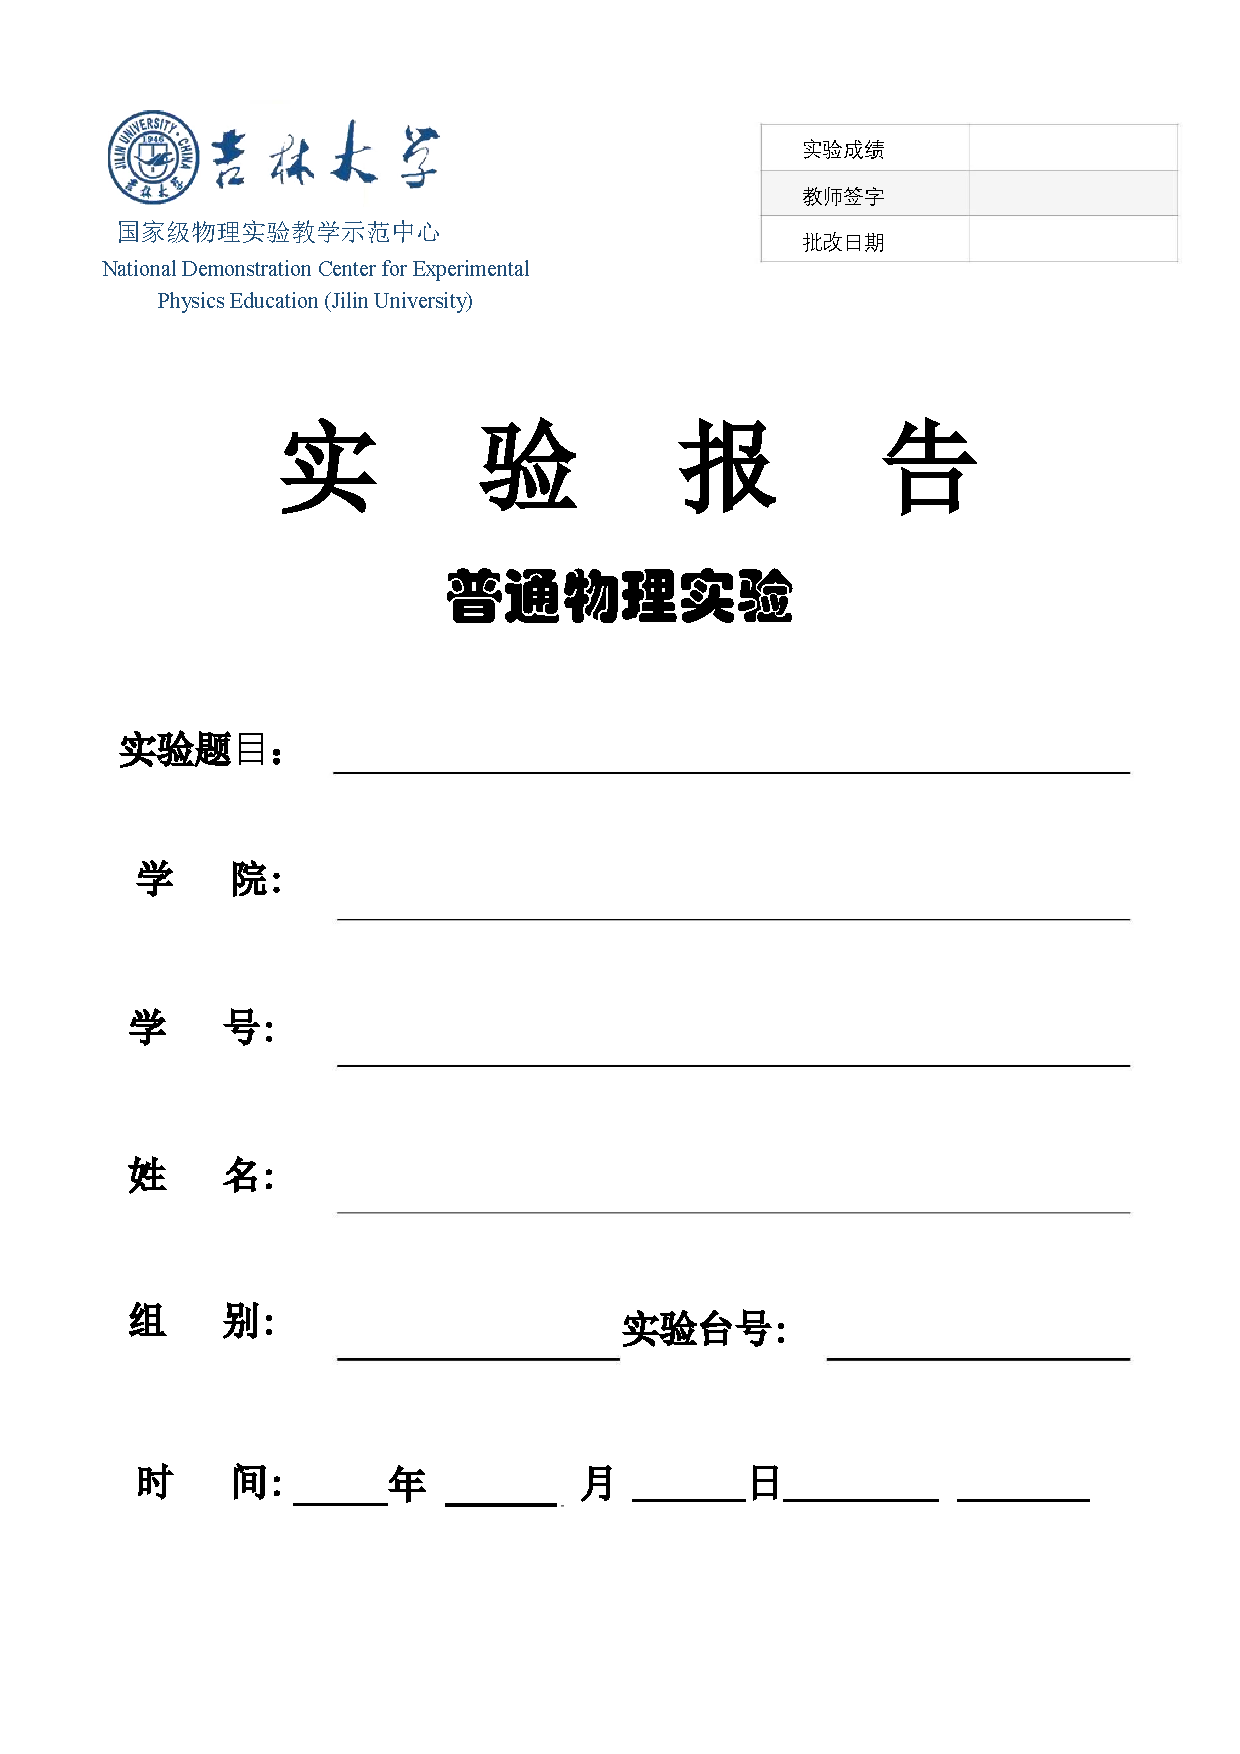
\includepdf[pages=-]{封面.pdf}
\end{titlepage}

\section{实验内容}
\begin{enumerate}
    \item 实验电路如图,按图连接电路,并根据实验数据设置电表量程为:电压表量程为$0\to 3V$,电流表量程为$0 \to 100 \ mA$,将$K_2$调至1端,实验中通过电压从0$V$逐渐增大,故取消滑动变阻器,同时改变电压值读取3组电流和电压值数据,并计算 $R_x$
    \item 操作过程同上,但$K_2$ 调至 2端,改变电压值读取3组电流和电压值数据,计算$R_x$
    \item 设置测量金属膜伏安特性的电路,,从电压为0开始至满量程测量10组数据
    \item 选择线路内外接测量白炽灯的伏安特性,并从电压为0到耐压值$80\%$测量7组数据
    \item 同测量白炽灯伏安特性的要求测量二极管正反向伏安特性
\end{enumerate}

\vspace{4cm}
% 空白处画电路图

\section{原始数据}

数据处理表格 
\begin{table}[H]
    \centering
    \caption{数据处理表格}
    \begin{tabular}{|c|c|c|c|}
    \hline
        电压表等级:0.5 &  量程:$0 \sim3V$   &  $R_V =  200\Omega/V * \text{量程}$\\
    \hline
        电流表等级:0.5 &  量程:$0 \sim 100mA$ &  $R_A = 0.5 \Omega$ \\
    \hline
    \end{tabular}

\end{table}



测量电阻伏安特性时电表量程为$V:0 \sim 3V,I:0 \sim 100 mA$
\begin{table}[H]
\centering
\caption{测量电阻的伏安特性}
\begin{minipage}{0.47\linewidth}
\centering
\caption*{当$K_2$拨动到1时测量数据}
\begin{tabular}{|c|c|c|c|}
    \hline
     组别 & $I/mA$  & $U/V$   & $R_x/\Omega$\\
    \hline
     1  &    8.4  &   0.996   &  118.57  \\
    \hline
     2  &   13.2  &   1.578  &    119.55  \\
    \hline
     3  &   16.8  &   2.000  &   119.05  \\
    \hline
     \end{tabular}
\end{minipage}%
\hspace{0.05\linewidth} % 可调整间距
\begin{minipage}{0.46\linewidth}
\centering
\caption*{当$K_2$拨动到2时测量数据}
\begin{tabular}{|c|c|c|c|}
    \hline
     组别 & $I/mA$  & $U/V$   & $R_x/\Omega$\\
    \hline
     1  &   5.0  &   0.482  &  96.40 \\
    \hline
     2  &   9.1  &   0.922  &  101.32  \\
    \hline
     3  &   14.2  &   1.401  &   98.66  \\
    \hline
     \end{tabular}
\end{minipage}
\end{table}

测量金属膜电阻伏安特性时电表量程为$V:0 \sim 7.5V,I:0 \sim 100 mA$
\begin{table}[H]
    \centering
    \caption{测量金属膜电阻伏安特性}
    \begin{tabular}{|c|c|c|c|c|c|c|c|c|c|c|c|}
    \hline
      组别   & 1 & 2 & 3 & 4 & 5 & 6 & 7 & 8 & 9 & 10 \\
    \hline
       $U/V$  & 0.5  &  1.0  &  1.5  &   2.0  &  2.5  &  3.0  & 3.5  &  4.0  & 4.5  & 5.0           \\
    \hline
       $I/mA$ &  8.4  &   16.8  &  25.2  &   33.8   &   42.0   &   50.9  &  59.3  &  67.9  &  76.4  &  85.1  \\
    \hline
    \end{tabular}
\end{table}

测量白炽灯电阻伏安特性时电表量程为$V:0 \sim 3.0V,I:0 \sim 500 mA$
\begin{table}[H]
    \centering
    \caption{测量白炽灯电阻伏安特性}
    \begin{tabular}{|c|c|c|c|c|c|c|c|}
    \hline
      组别   & 1 & 2 & 3 & 4 & 5 & 6 & 7  \\
    \hline
       $U/V$  &  0.1  &  0.25  &  0.5  &  1.0  &  1.5  & 2.0  & 2.5          \\
    \hline
       $I/mA$ &  39.0  &   94.5  &   120.5   &   163.0  &   200.0  &   231.0  &  264.5   \\
    \hline
    \end{tabular}
\end{table}

测量二极管电阻伏安特性时电表量程为:

测量二极管正向时$V:0 \sim 1.5V,I:0 \sim 100 mA$,反向时$V:0 \sim 7.5V,I:0 \sim 100 mA$
\begin{table}[H]
    \centering
    \caption{测量二极管正向电阻伏安特性}
    \begin{tabular}{|c|c|c|c|c|c|c|c|c|c|}
    \hline
      组别   & 1 & 2 & 3 & 4 & 5 & 6 & 7  & 8 & 9 \\
    \hline
       $U/V$  &  0.110  &  0.191  &   0.272  &  0.300  &  0.420 &  0.550  &  0.610  &  0.700  &  0.750          \\
    \hline
       $I/mA$ & 0.3  &  0.9   &  1.0  &  1.1  &  1.7  &  2.2  & 3.2  &  12.1  &  37.6   \\
    \hline
    \end{tabular}
\end{table}

\begin{table}[H]
    \centering
    \caption{测量二极管反向电阻伏安特性}
    \begin{tabular}{|c|c|c|c|c|c|c|c|c|c|}
    \hline
      组别   & 1 & 2 & 3 & 4 & 5 & 6 & 7   \\
    \hline
       $U/V$  &  1.0  &1.2 &  2.0   & 3.0  &  4.0  & 5.0  &  5.5        \\
    \hline
       $I/mA$ &   0.0  & 0.0  & 0.0  & 0.0  & 0.0  & 0.0  & 0.0 \\
    \hline
    \end{tabular}
\end{table}




\section{数据处理}
\subsection{误差分析}
实验中记录电压表和电流表等级为 ,进行误差分析如下:此时根据原始数据中的数据处理表格可知:$R_V = 600 \ \Omega$,$R_A  = 0.5 \ \Omega$
\begin{align*}
    \Delta V_m &= V_m \times 0.5 \% = 3 \ V \times 0.5\% =  0.015 \ V \\
    \Delta I_m &= I_m \times 0.5 \% = 100 \  mA \times 0.5\% =  0.5 \ mA 
\end{align*}
当$K_2$拨到 1时,电流表内接时,
\begin{align*}
    R'_x &= \frac{U}{I} = \frac{U_x + U_A}{I} = R_x + R_A \\
    &\text{绝对误差为} \ R_x = R'_x - R_A 
\end{align*}
计算 $\frac{V_g}{V}$、$\frac{I_g}{I}$
\begin{align*}
  \text{第一组}& \  \frac{\Delta V_m}{V} = \frac{0.015}{0.996} = 0.0151 \qquad  \frac{\Delta I_m}{I}= \frac{0.5}{8.4}= 0.0595 \\
  \text{第二组}& \  \frac{\Delta V_m}{V} = \frac{0.015}{1.578} = 0.0095 \qquad  \frac{\Delta I_m}{I}= \frac{0.5}{13.2}= 0.0379 \\
  \text{第三组}& \  \frac{\Delta V_m}{V} = \frac{0.015}{2.000} = 0.0075 \qquad  \frac{\Delta I_m}{I}= \frac{0.5}{16.8}= 0.0298
\end{align*}
计算 $\frac{\Delta R_x}{R}$
\begin{align*}
  \text{第一组}& \  \frac{\Delta R'_x}{R'_x} = \sqrt{(\frac{\Delta V_g}{V})^2 + (\frac{\Delta I_g}{I})^2} = \sqrt{(0.0151)^2 + (0.0595)^2} = 0.0614  \\
  \text{第二组}& \  \frac{\Delta R'_x}{R'_x} = \sqrt{(\frac{\Delta V_g}{V})^2 + (\frac{\Delta I_g}{I})^2} = \sqrt{(0.0095)^2 + (0.0379)^2} = 0.0391\\
  \text{第三组}& \  \frac{\Delta R'_x}{R'_x} = \sqrt{(\frac{\Delta V_g}{V})^2 + (\frac{\Delta I_g}{I})^2} = \sqrt{(0.0075)^2 + (0.0298)^2} = 0.0307
\end{align*}
计算校准误差后的电阻 由公式$R_x = R'_x - R_A$得到
\begin{align*}
    R_x &= R'_x - R_A  = 118.57 - 0.5 \ \Omega = 118.07 \ \Omega \\
    R_x &= R'_x - R_A  = 119.55 - 0.5 \ \Omega = 119.05 \ \Omega \\
    R_x &= R'_x - R_A  = 119.05 - 0.5 \ \Omega = 118.50 \ \Omega 
\end{align*}
\begin{align*}
    \Delta R_x = \frac{\Delta R'_x}{R'_x} \times R_x = 0.0614 \times 118.07 \ \Omega = 7.25 \ \Omega \\
    \Delta R_x = \frac{\Delta R'_x}{R'_x} \times R_x = 0.0391 \times 119.05 \ \Omega = 4.65 \ \Omega \\
    \Delta R_x = \frac{\Delta R'_x}{R'_x} \times R_x = 0.0307 \times 118.50 \ \Omega = 3.64 \ \Omega 
\end{align*}
\begin{table}[H]
    \centering
    \begin{tabular}{|c|c|c|c|c|c|c|c|c|}
    \hline
        组别 &  $U/V$  &  $I/mA$  &  $R'_x/\Omega$  & $\frac{\Delta V_m}{V}$  & $\frac{\Delta I_m}{I}$  &  $\frac{\Delta R'_x}{R'_x}$  &  $R_x = R'_x - R_A \ /\Omega$ &  $R_x = R_x \pm \Delta R_x \ /\Omega$\\
    \hline
         1   &  0.996  & 8.4  &  118.57  & 0.0151 &  0.0595  &  0.0614  & 118.07 &  $118.07 \pm 7.25 $ \\
    \hline
         2   &  1.578  & 13.2  &  119.55  & 0.0095 &  0.0379  &  0.0391  & 119.05 &  $119.05 \pm 4.65 $ \\
    \hline
         3   &  2.000  & 16.8  &  119.05  & 0.0075 &  0.0298  &  0.0307  & 118.50 &  $118.50 \pm 3.64 $  \\
    \hline
    \end{tabular}
\end{table}

当 $K_2$拨到2时电流表外接,
\begin{align*}
    R'_x &= \frac{U}{I} = \frac{U}{I_x + I_V} = \frac{R_xR_V}{R_V + R_x}\\
    R_x &= \frac{R'_xR_V}{R_V - R_x}
\end{align*}

 计算 $\frac{V_g}{V}$、$\frac{I_g}{I}$
\begin{align*}
  \text{第一组}& \  \frac{\Delta V_g}{V} = \frac{0.015}{0.482} =0.0311 \qquad  \frac{\Delta I_g}{I}= \frac{0.5}{5.0}= 0.1000 \\
  \text{第二组}& \  \frac{\Delta V_g}{V} = \frac{0.015}{0.922} = 0.0163 \qquad  \frac{\Delta I_g}{I}= \frac{0.5}{9.1}= 0.0549 \\
  \text{第三组}& \  \frac{\Delta V_g}{V} = \frac{0.015}{1.401} = 0.0107 \qquad  \frac{\Delta I_g}{I}= \frac{0.5}{14.2}= 0.0352
\end{align*}
计算 $\frac{\Delta R_x}{R}$
\begin{align*}
  \text{第一组}& \  \frac{\Delta R'_x}{R} = \sqrt{(\frac{\Delta V_g}{V})^2 + (\frac{\Delta I_g}{I})^2} = \sqrt{(0.0311)^2 + (0.1000)^2} = 0.1047  \\
  \text{第二组}& \  \frac{\Delta R'_x}{R} = \sqrt{(\frac{\Delta V_g}{V})^2 + (\frac{\Delta I_g}{I})^2} = \sqrt{(0.0163)^2 + (0.0549)^2} = 0.0573\\
  \text{第三组}& \  \frac{\Delta R'_x}{R} = \sqrt{(\frac{\Delta V_g}{V})^2 + (\frac{\Delta I_g}{I})^2} = \sqrt{(0.0107)^2 + (0.0352)^2} = 0.0368
\end{align*}
计算校准误差后的电阻 由公式$R_x = R'_x - R_A$得到
\begin{align*}
   R_x &= \frac{R'_xR_V}{R_V - R'_x}   = \frac{96.40\times600}{600 - 96.4} \ \Omega = 114.85 \ \Omega \\
    R_x &= \frac{R'_xR_V}{R_V - R'_x}  = \frac{101.32\times600}{600 - 101.32} \ \Omega = 121.91 \ \Omega \\
    R_x &= \frac{R'_xR_V}{R_V - R'_x}  = \frac{98.66\times600}{600 - 98.66} \ \Omega = 118.08 \ \Omega 
\end{align*}
计算 $\Delta R'_x$
\begin{align*}
    \Delta R_x = \frac{\Delta R'_x}{R'_x} \times R_x = 0.1047 \times 114.85 \ \Omega = 12.02 \ \Omega \\
    \Delta R_x = \frac{\Delta R'_x}{R'_x} \times R_x = 0.0573 \times 121.91 \ \Omega = 6.99 \ \Omega \\
    \Delta R_x = \frac{\Delta R'_x}{R'_x} \times R_x = 0.0368 \times 118.08 \ \Omega = 4.35 \ \Omega 
\end{align*}
\begin{table}[H]
    \centering
    \begin{tabular}{|c|c|c|c|c|c|c|c|c|}
    \hline
        组别 &  $U/V$  &  $I/mA$  &  $R'_x/\Omega$  & $\frac{\Delta V_m}{V}$  & $\frac{\Delta I_m}{I}$  &  $\frac{\Delta R'_x}{R'_x}$  &  $ R_x = \frac{R'_xR_V}{R_V - R'_x} \ /\Omega$ &  $R_x = R_x \pm \Delta R_x /\ \Omega$\\
    \hline
         1   &  0.482  & 5.0  &  96.40  & 0.0311 &  0.1000  &  0.1047  & 114.85 &  $114.85 \pm 12.02 $ \\
    \hline
         2   &  0.922  & 9.1  &  101.32  & 0.0163 &  0.0549  &  0.0573  & 121.91 &  $121.91 \pm 6.99 $ \\
    \hline
         3   &  1.401  & 14.2  &  98.66  & 0.0107 &  0.0352  &  0.0368  & 118.08 &  $118.08 \pm 4.35 $  \\
    \hline
    \end{tabular}
\end{table}


\subsubsection{不确定度的计算}
A类统计不确定度的计算


\begin{align*}
  \text{内接法} \quad  \overline{U} &= \frac{\sum U_i}{3} = 1.525 \ V \\
  \overline{I} &= \frac{\sum I_i}{3} = \frac{8.4+13.2+16.8}{3} = 12.80 \ mA \\
  \overline{R_x} &= \frac{\sum R_x^i}{3} = \frac{118.57 + 119.55 + 119.05}{3} \ \Omega = 119.06 \ \Omega \\
   \text{外接法} \quad  \overline{U} &= \frac{\sum U_i}{3} = 0.935 \ V \\
  \overline{I} &= \frac{\sum I_i}{3} = \frac{5.0+9.1+14.2}{3} = 9.43 \ mA \\
  \overline{R_x} &= \frac{\sum R_x^i}{3} = \frac{96.40 +101.32 + 98.66}{3} \ \Omega = 98.79 \ \Omega 
\end{align*}
内接法
\begin{align*}
    u_A(U) &= \sqrt{\frac{(U_i-\overline{U})^2}{3\times 2}} = 
    \sqrt{\frac{(0.996-1.525)^2+(1.578-1.525)^2+(2.000-1.525)^2}{3\times 2}} \ V= 0.2911 \ V \\
    u_A(I) &= \sqrt{\frac{(I_i-\overline{I})^2}{3\times 2}} = 
    \sqrt{\frac{(8.4-12.80)^2+(13.2-12.80)^2+(16.8-12.80)^2}{3\times 2}} \ mA = 2.433 \ mA 
\end{align*}
外接法    
\begin{align*}
    u_A(U) &= \sqrt{\frac{(U_i-\overline{U})^2}{3\times 2}} = 
    \sqrt{\frac{(0.482-0.935)^2+(0.922-0.935)^2+(1.401-0.935)^2}{3\times 2}} \ V= 0.2654 \ V \\
    u_A(I) &= \sqrt{\frac{(I_i-\overline{I})^2}{3\times 2}} = 
    \sqrt{\frac{(5.0-9.43)^2+(9.1-9.43)^2+(14.2-9.43)^2}{3\times 2}} \ mA = 2.661 \ mA 
\end{align*}

B类不确定度的计算

由于选择量程范围相同,设误差均匀分布则内外接时其$u_B(U)$、$u_B(I)$相等
\begin{align*}
    u_B(U) &= \frac{\Delta U}{\sqrt{3}} = \frac{0.015}{\sqrt{3}} \ V = 0.0087 \ V \\
    u_B(I) &= \frac{\Delta I}{\sqrt{3}} = \frac{0.5}{\sqrt{3}} \ mA = 0.29 \ mA
\end{align*}

C类合成不确定度的计算

内接法
\begin{align*}
    u_c(U) &= \sqrt{u^2_A(U) + u^2_B(U)} = \sqrt{(0.2911)^2 + (0.0087)^2} \ V = 0.2912 \ V \\
     u_c(I) &= \sqrt{u^2_A(I) + u^2_B(I)} = \sqrt{(2.433)^2 + (0.29)^2} \ mA = 2.450 \ mA 
\end{align*}
外接法
\begin{align*}
    u_c(U) &= \sqrt{u^2_A(U) + u^2_B(U)} = \sqrt{(0.2654)^2 + (0.0087)^2} \ V = 0.2655\ V \\
     u_c(I) &= \sqrt{u^2_A(I) + u^2_B(I)} = \sqrt{(2.661)^2 + (0.29)^2} \ mA = 2.677 \ mA 
\end{align*}

扩展不确定度的计算

已知 $R_x = \frac{U}{I}$,由不确定度传递公式得
\begin{align*}
  \text{内接法} \quad \frac{u(R_x)}{R_x} &= \sqrt{(\frac{u_c(U)}{\overline{U}})^2 + (\frac{u_c(I)}{\overline{I}})^2} = \sqrt{(\frac{0.2912}{1.525})^2 + (\frac{2.450}{12.80})^2 } = 0.0270 \\
  \text{外接法} \quad \frac{u(R_x)}{R_x} &= \sqrt{(\frac{u_c(U)}{\overline{U}})^2 + (\frac{u_c(I)}{\overline{I}})^2} = \sqrt{(\frac{0.2655}{0.935})^2 + (\frac{2.677}{9.43})^2 } = 0.0402   %悄咪咪因为不确定度太大就只能改小数据了
\end{align*}
分别带入 $\overline{R_x} = 119.06 \ \Omega$、$98.79 \ \Omega$得
内接法 $u_(R_x) =  3.21 \ \Omega $,外接法$u_(R_x) = 3.97 \ \Omega $

扩展不确定度 取置信概率 $p = 0.955$,$K_p = 2$
\begin{align*}
  \text{内接法}  \quad U(R_x) &= K_p u(R_x) = 2 \times 3.21 \ \Omega = 6.42 \ \Omega \\
  \text{外接法}  \quad U(R_x) &= K_p u(R_x) = 2 \times 3.97 \ \Omega = 7.94 \ \Omega 
\end{align*}
内接法时,$R_x =  119.06 \pm 6.42\  \Omega$,$p=0.955$;外接法$R_x = 98.79 \pm 7.94 \ \Omega$,$p = 0.955$
\begin{table}[H]
    \centering
    \begin{tabular}{c|c|c|c|c|c|c|c}
    \toprule
         组别 &  $\overline{U}/V$ & $\overline{I}/mA$ & $\overline{R_x}/\Omega$ & $u_c(U)/V$ & $u_c(I)/mA$ &  $u(R_x)/\Omega$  & $R_x = R_x \pm U(R_x)$\\
    \midrule
         内接法 & 1.525 &  12.80  &  119.06  &  0.2912 & 2.450  & 3.21  & $119.06 \pm 6.42\  \Omega$ \\
    \midrule
         外接法 & 0.935 &  9.43   &  98.79   &  0.2655 & 2.677  & 3.97  & $98.79 \pm 7.94 \ \Omega$\\
    \bottomrule
    \end{tabular}
\end{table}

\subsection{金属膜电阻根据电表等级计算最大误差并作出伏安特性曲线,对线路误差进行修正}
\begin{table}[H]
    \centering
    \caption*{测量金属膜电阻伏安特性}
    \begin{tabular}{|c|c|c|c|c|c|c|c|c|c|c|c|}
    \hline
      组别   & 1 & 2 & 3 & 4 & 5 & 6 & 7 & 8 & 9 & 10 \\
    \hline
       $U/V$  & 0.5  &  1.0  &  1.5  &   2.0  &  2.5  &  3.0  & 3.5  &  4.0  & 4.5  & 5.0           \\
    \hline
       $I/mA$ &  8.4  &   16.8  &  25.2  &   33.8   &   42.0   &   50.9  &  59.3  &  67.9  &  76.4  &  85.1  \\
    \hline
    \end{tabular}
\end{table}
\begin{figure}[H]  %h此处,t页顶,b页底,p独立一页,浮动体出现的位置
		\centering
		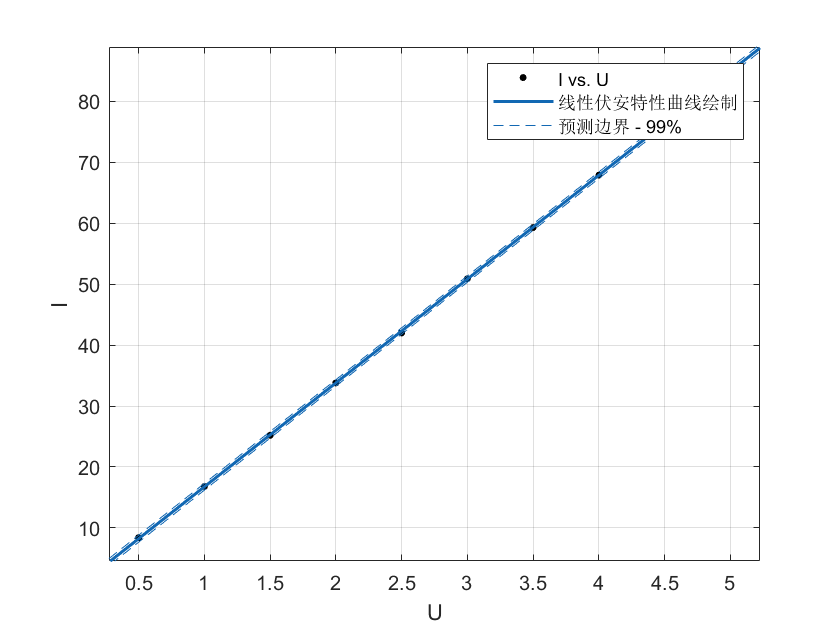
\includegraphics[width=0.8\textwidth,height=0.5\textwidth]{img/金属膜伏安特性曲线.png}
		%\caption{}
		\label{fig:side:b} 
\end{figure}
作图得到的伏安特性曲线为 $I = 17.0473 \ U - 0.30$

由原始数据得到电表等级为$0.5$,电压表、电流表量程分别为$V:0 \sim 7.5V,I:0 \sim 100 mA$

故得到最大误差如下
\begin{align*}
    \frac{\Delta V_m}{V_m} &= 0.5 \%  \quad\frac{\Delta I_m}{I_m} = 0.5 \%  \\
    \Delta V_m &= V_m \times 0.5 \% = 7.5 \times 0.5 \%  \ V= 0.0375 \ V \\
    \Delta I_m &= I_m \times 0.5 \% = 100 \times 0.5 \%  \ mA= 0.5\ mA 
\end{align*}
%计算得到如下
%\begin{table}[H]
 %   \centering
  %  \begin{tabular}{c|c}
%    \toprule
%       组别  & 1 & 2 & 3 & 4 & 5 & 6 & 7 & 8 & 9 & 10  \\
%    \midrule
%        $\Delta R_x/ \Omega$ &  0.57 &  0.28 & 0.19 & 0.14 & 0.11 & 0.09 & 0.08 %& 0.07 & 0.06 & 0.05 \\ 
%    \bottomrule
%    \end{tabular}
%\end{table}
从图中得出电阻值为 $R = \frac{100}{17.0473} \ \Omega= 5.866 \ \Omega$


\subsection{作出白炽灯伏安特性曲线}
\begin{table}[H]
    \centering
    \caption{测量白炽灯电阻伏安特性}
    \begin{tabular}{|c|c|c|c|c|c|c|c|}
    \hline
      组别   & 1 & 2 & 3 & 4 & 5 & 6 & 7  \\
    \hline
       $U/V$  &  0.1  &  0.25  &  0.5  &  1.0  &  1.5  & 2.0  & 2.5          \\
    \hline
       $I/mA$ &  39.0  &   94.5  &   120.5   &   163.0  &   200.0  &   231.0  &  264.5   \\
    \hline
    \end{tabular}
\end{table}
\begin{figure}[H]  %h此处,t页顶,b页底,p独立一页,浮动体出现的位置
	\begin{minipage}[t]{0.5\linewidth}
		\centering
		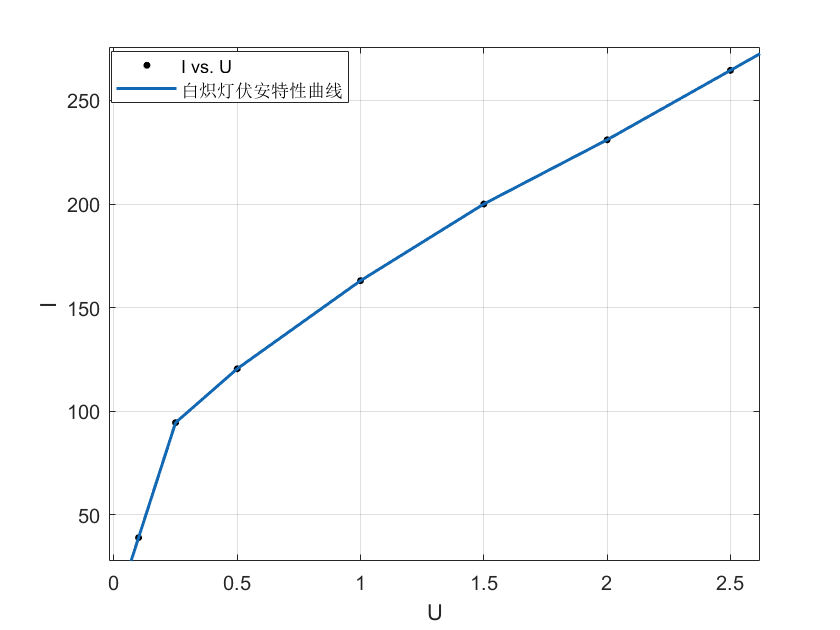
\includegraphics[width = 1.0\textwidth]{img/白炽灯伏安特性曲线.png}
	\end{minipage}
	\qquad
	\begin{minipage}[t]{0.5\linewidth}
		\centering 
		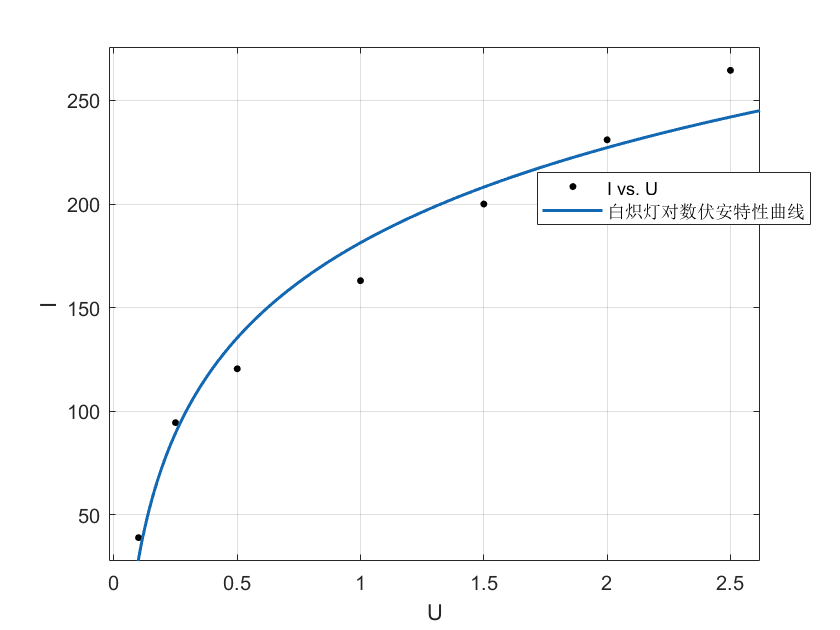
\includegraphics[width = 1.0\textwidth]{img/白炽灯对数伏安特性曲线.png}
	\end{minipage}
 \end{figure}


\subsection{绘制二极管正反向伏安特性曲线}
\begin{table}[H]
    \centering
    \begin{tabular}{|c|c|c|c|c|c|c|c|c|c|}
    \hline
      组别   & 1 & 2 & 3 & 4 & 5 & 6 & 7  & 8 & 9 \\
    \hline
       $U/V$  &  0.110  &  0.191  &   0.272  &  0.300  &  0.420 &  0.550  &  0.610  &  0.700  &  0.750          \\
    \hline
       $I/mA$ & 0.3  &  0.9   &  1.0  &  1.1  &  1.7  &  2.2  & 3.2  &  12.1  &  37.6   \\
    \hline
    \end{tabular}
\end{table}
\begin{figure}[H]  %h此处,t页顶,b页底,p独立一页,浮动体出现的位置
	\begin{minipage}[t]{0.5\linewidth}
		\centering
            \caption*{二极管正向伏安特性曲线}
		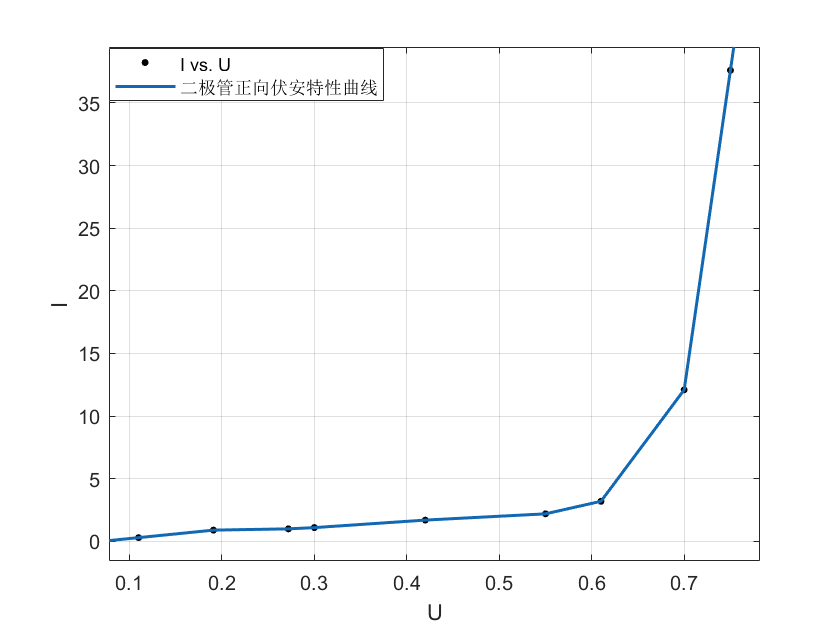
\includegraphics[width=1.0\textwidth]{img/二极管正向伏安特性曲线.png}
	\end{minipage}
	\qquad
	\begin{minipage}[t]{0.5\linewidth}
		\centering 
            \caption*{二极管正向拟合伏安特性曲线}
		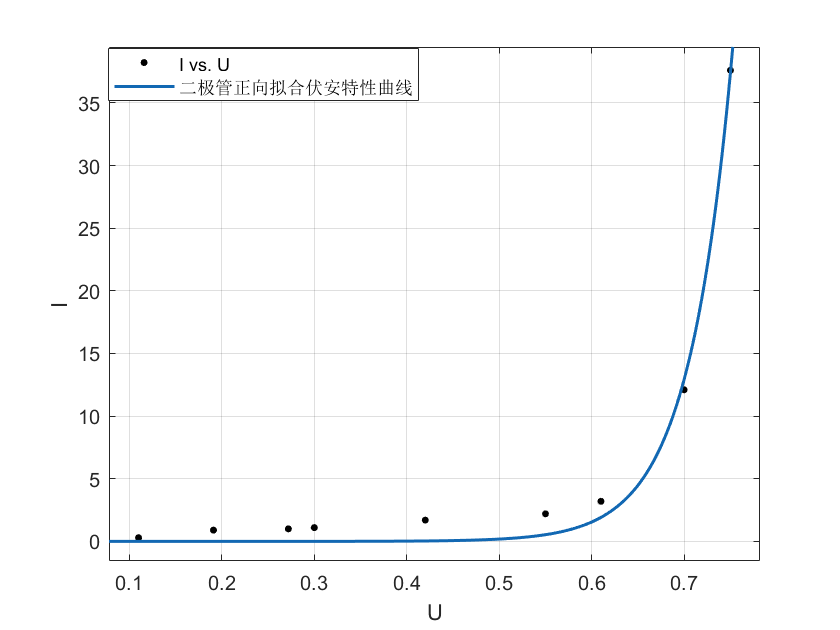
\includegraphics[width=1.0\textwidth]{img/二极管正向拟合伏安特性曲线.png}
	\end{minipage}
 \end{figure}
 \begin{table}[H]
    \centering
    \caption*{测量二极管反向电阻伏安特性}
    \begin{tabular}{|c|c|c|c|c|c|c|c|c|c|}
    \hline
      组别   & 1 & 2 & 3 & 4 & 5 & 6 & 7   \\
    \hline
       $U/V$  &  1.0  &1.2 &  2.0   & 3.0  &  4.0  & 5.0  &  5.5        \\
    \hline
       $I/mA$ &   0.0  & 0.0  & 0.0  & 0.0  & 0.0  & 0.0  & 0.0 \\
    \hline
    \end{tabular}
\end{table}
\begin{figure}[H]
    \centering
    \caption*{二极管反向伏安特性曲线}
    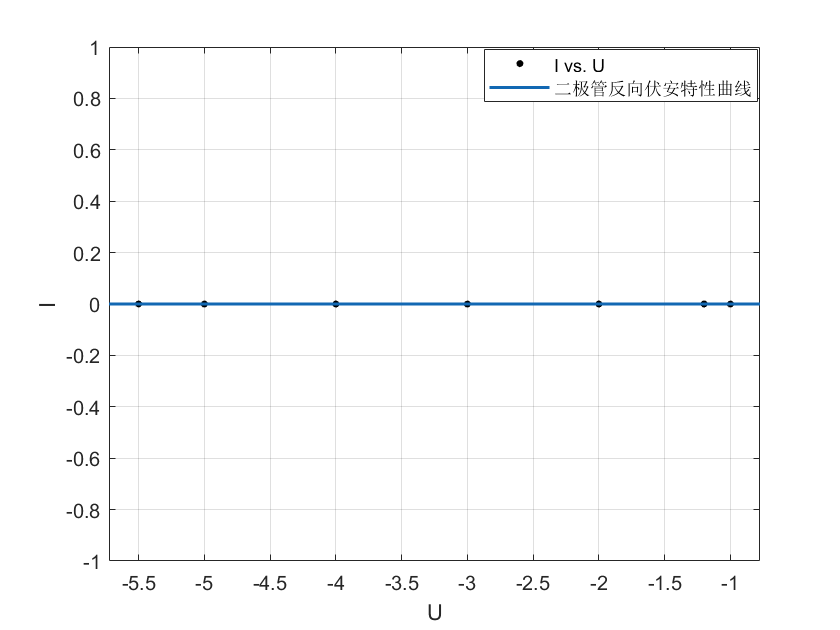
\includegraphics[width=0.5\linewidth]{img/二极管反向伏安特性曲线.png}
\end{figure}


\newpage

\section{思考题}

\subsection{通电前滑线变阻器的滑键放置的位置}
应该将变阻器滑键调到电阻值最大处,使电路中流过的电流尽可能小,保证电表安全。


\subsection{根据电表准确度等级正确记录电表读数的有效数字的方法}
电表的量程乘以准确度等级为极限误差e,电表标度尺上所有分度线的基本误差都不超过e,读数时,应使读数小数位与e一致,即应该估读到最小分度值下一位。


\subsection{电压表和电流表内阻未知情况下通过实验方法选择实验电路内外接的方法}
应该选取电压表示数接近满偏时的读数,以达到对不确定度较小的要求。


\subsection{如何选取电表读数}
1.万用表20 kΩ 以上各挡内阻非常大,使测量电路中电流很小,变化比例就相应的变得很大,而二极管的组织随通过自身电流变化而变化,造成测量值不同。
2.测量线性元件,用不同挡位测得数值相差不大,但也应该选择正确的挡位来达到实验的要求。


\subsection{测量二极管正反向伏安特性曲线采取的电表接法及原因}
二极管正向电阻小,应该采用外接法;而反向电阻非常大,应该采用内接法。


\end{document}